\chapter{Existující nástroje}
\label{3-nastroje}

Tato kapitola se zabývá již existujícími nástroji pro spojování vektorových map
 z~různých zdrojů (\textit{conflation}).


\section{Proprietární nástroje}
\label{proprietární}

Proprietárních nástrojů umožňujících řešení spojování vektorových map 
existuje celá řada. Některé programy jsou orientovány přímo na~tento problém,
jiné nabízejí funkce pro slučování map pouze jako vedlejší funkcionalitu 
a~ne vždy je proto možné pomocí nich řešit složitější problémy. Následující
výčet neobsahuje všechen komerční software zabývající se slučováním
vektorových map, ale nejvýznamnější nástroje, které lze pro zpracování 
použít. Vzhledem k~tomu, že se jedná o~proprietární software, nebylo možné 
všechny níže popsané nástroje otestovat, proto jejich popis vychází 
především z~informací dostupných na~oficiálních internetových stránkách 
produktů.


\subsection{ESRI ArcGIS}
\label{arcgis}

V~softwaru ArcGIS 10\footnote{\url{http://www.esri.com/software/arcgis}} 
existuje několik nástrojů, které lze využít pro spojování
geo\-grafických dat, přenos atributů a~odstraňování geometrických rozdílů 
mezi datasety. 

\subsubsection{Spatial Adjustment}

Soubor nástrojů \textit{Spatial Adjustment} systému ArcGIS zahrnuje 
základní funkce týkající se této problematiky. Má sloužit především 
k~úpravě dat z~různých zdrojů a~zajistit tak jejich celistvost. 
Poskytuje několik metod pro zarovnání jedné vrstvy či její části 
ke~druhé. Lze provést transformaci, navázání hran (\textit{edge matching})
nebo srovnání překrývajících se dat (\textit{rubber sheeting}).

Pro použití metody transformace je nejdříve třeba označit data, která budou
do~procesu vstupovat. Poté se vyberou dvojice uzlových bodů, které by si měly
odpovídat. Na~výběr je několik typů transformací pro úpravu dat
na~zá\-kladě vybraných dvojic identických bodů. 

Do~procesu horizontálního zarovnání (\textit{horizontal conflation}) lze 
zařadit funkce nástroje \textit{Edge Match Tool}, který umožňuje navázat 
na~sebe dvě sousedící vrstvy. Zarovnání je poměrně snadné, stačí pouze 
zvolit toleranci (maximální vzdálenost pro navázání prvků) a~označit tímto
nástrojem hranici mezi vrstvami, kde by měly na~sebe navazovat. Ve~vybrané
oblasti se zobrazí indikátory naznačující způsob zarovnání, které lze ještě
ručně upravit. Po~potvrzení se provede zarovnání tak, aby byla zachována
topologie.

Dalším způsobem geometrického spojení vrstev, který \textit{Spatial Adjustment}
nabízí, je \textit{Rubber Sheeting}. V~tomto případě je opět třeba označit 
odpovídající si body a~navíc body, jejichž poloha by se neměla změnit. 
Při~spuštění zarovnání se dočasně vytvoří triangulační síť mezi označenými body. 
Poloha ostatních neoznačených bodů je pak vypočtena interpolací v~trojúhelnícíh 
sítě.

Poslední z~nástrojů pro kombinaci map je \textit{Attribute Transfer}. Pomocí 
něho je možné převést atributy mezi odpovídajícími si prvky, ale také upravit
jejich geometrii. Po~volbě jednoho či více atributů, které se mají převádět 
mezi zdrojovou a~cílovou vrstvou lze interaktivně vybírat odpovídající si 
dvojice prvků v~obou vrstvách. Mezi~těmito prvky se převedou atributy a~pokud
je zaškrtnuta volba \textit{Transfer Geometry} neboli \uv{převést geometrii},
změní se geometrie cílového prvku dle~zdrojového. Převod lze provést také 
najednou pro více vybraných prvků.

\subsubsection{Integrate}

  \begin{figure}[H]
    \centering
      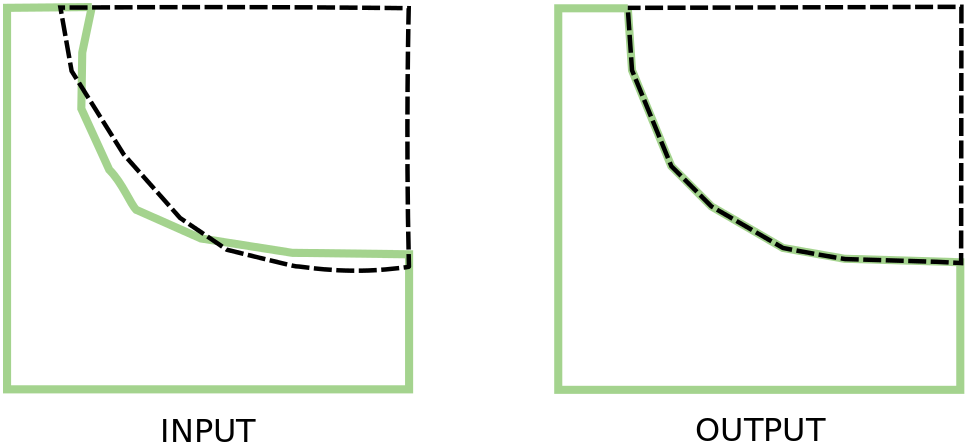
\includegraphics[width=250pt]{./pictures/integrate.png}
      \caption[Integrate - princip]{Integrate - princip 
	  (zdroj: \url{http://resources.arcgis.com/en/help/main/10.1/index.html\#//00170000002s000000})}
      \label{fig:integrate}
  \end{figure}

Nástroj \textit{Integrate} umožňuje sladění dvou datasetů. Na~vstupu vyžaduje 
dvě či více vrstev, které chceme zarovnat, a~dále maximální vzdálenost, při~které
lze považovat prvky za~odpo\-vídající si. U~každého datasetu navíc lze zadat 
prioritu (\textit{rank}). Prvky s~nižší prioritou se pak budou zarovnávat 
k~těm s~prioritou vyšší. Tato funkce je velmi užitečná, pokud máme dvě 
překrývající se nebo sousedící vrstvy s~malými rozdíly např. v~důsledku různé
přesnosti.


\subsection{ConfleX}
\label{conflex}

ConfleX\footnote{\url{http://www.citygategis.com/conflex.htm}} 
je software pro automatické spojování vektorových \zk{GIS} dat,
který pro automatizaci využívá umělou inteligenci. ConfleX umožňuje zpracování 
i~takových případů, kdy se zdrojová mapa s~cílovou nepřekrývají nebo nejsou 
topologicky identické. Systém porovnává každé dva segmenty z~obou map a~jejich
vztah k~ostatním segmentům. Na~základě tohoto postupu pak rozhodne, zda se 
jedná o~stejné prvky či nikoli. Kromě automatického procesu umožňuje program 
i~následnou ruční editaci.

ConfleX je k~dispozici jako samostatná aplikace ale také jako extenze 
programu ArcGIS Desktop 9/10.


\subsection{Intergraph GeoMedia Fusion}
\label{geomedia}

Jedná se o~doplněk desktopové aplikace 
GeoMedia\footnote{\url{http://geospatial.intergraph.com/products/GeoMedia/Details.aspx}}
firmy Intergraph, který je dostupný od~roku 2005. Nástroj GeoMedia Fusion  
je navržen pro topologické opravy dat, validaci atributů a~integraci dat. Cílem 
je umožnit snadnou údržbu dat v~rozsáhlých geografických databázích, kde jsou 
data získávána z~různých zdrojů. Nástroj porovnává dva datasety obsahující 
rozdílné reprezentace stejné skutečnosti. Nejdříve automaticky vytvoří 
\textit{conflation links} indikující způsob spojení vrstev, které lze ještě
ručně editovat. Následně geometrie i~atributy těchto dvou reprezentací
sjednotí. GeoMedia Fusion slouží k~úpravě bodových, liniových i~plošných dat
včetně jejich atributů. 


\subsection{MapMerger}
\label{mapmerger}

MapMerger\footnote{\url{http://www.mapmerger.com}} je \zk{GIS} nástroj firmy 
ESEA zaměřený na~slučování geometrie a~atributů vektorových map a~kontrolu 
kvality dat. Umožňuje převod atributů mezi dvěma překrývajícími se mapami, 
navázání hranic dvou sousedících map, přidání prvků z~jedné mapy do~druhé, 
synchronizaci mapy s~její aktualizovanou verzí, identifikaci geometrických 
a~atributových rozdílů mezi dvěma verzemi té samé mapy. První verze programu 
vyšla již v~roce 1998, od~té doby již firma vyvinula 9~verzí. Z~uvedených 
nástrojů poskytuje asi nejvíce možností zpracování a~díky specializaci 
přímo na~spojování map se řadí mezi nejvýkonnější programy v~této oblasti. 


\section{Open Source nástroje}
\label{open-source}

V~této sféře zatím neexistuje mnoho nástrojů, které by komplexně řešili problém
spojování vektorových map (\textit{conflation}). Většinou jde pouze o~malé 
programy či zásuvné moduly k~větším projektům, pomocí nichž se dá provést manuální
nebo poloautomatické sloučení vektorových datasetů, případně jejich atributů. 
Ovšem většinou je cesta k~dosažení cíle pomocí těchto nástrojů poměrně složitá 
a~ne vždy jsou výsledky takové, jak bychom si představovali. Asi jediným 
ucelenějším nástrojem je knihovna \zkratka{JCS} implementovaná jako kolekce 
zásuvných modulů v~programu OpenJUMP.


\subsection{JCS - Java Conflation Suite}
\label{jcs}

\zk{JCS}\footnote{\url{http://www.vividsolutions.com/jcs/}} je \textit{open source}
knihovna napsaná v~jazyce Java, která zahrnuje API a~soubor interaktivních nástrojů, 
které slouží ke~slučování prostorových datasetů. Byla vyvinuta společností Vivid 
Solutions, Inc. Obsahuje funkce umožňující provádění různých procesů spojených 
se~spojování vektorových map, které jsou zaměřeny především na~polygonové, případně 
liniové datasety. Co se týče bodových vrstev, je její funkcionalita poměrně omezená. 
Knihovna \zk{JCS} je závislá na~knihovně 
\zkratka{JTS}\footnote{\url{http://www.vividsolutions.com/jts/}}, která poskytuje 
základní geometrické funkce pro práci s~prostorovými daty. Obě knihovny jsou navrženy 
v~souladu s~\zk{OGC} specifikací \textit{Simple Features} pro SQL,
která popisuje způsob uložení geografic\-kých digitálních dat, pro\-storové vztahy 
a~funkce. Knihovna \zk{JCS} vznikla v~rámci projektu JUMP Unified Mapping Platform. Je 
poskytována pod~licencí 
\zkratka{LGPL}\footnote{\url{http://www.gnu.org/licenses/lgpl.html}}.

\subsubsection{Architektura}

Knihovna \zk{JCS} používá pro vizualizaci dat a~interakci JUMP WorkBench
a~API. Poskytování základní geometrické funkcionality je pak zajištěno 
knihovnou \zk{JTS}. JUMP API umožňuje vstup a~výstup prostorových dat 
a~další funkcionalitu s~nimi spojenou. Jádro \zk{JCS} tvoří Conflation API
obsahující algoritmy pro kontrolu a~slučo\-vání prostorových dat 
(\textit{conflation}). Funkce \zk{JCS} jsou v~projektu OpenJUMP 
implementovány v~podobě kolekce zásuvných modulů - \textit{QA, Conflate, 
RoadMatcher}.

  \begin{figure}[H]
    \centering
      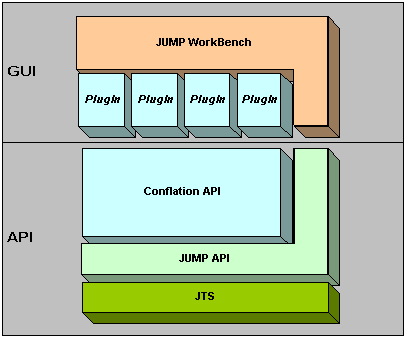
\includegraphics[width=280pt]{./pictures/JCS_Architecture.png}
      \caption[Architektura JCS]{Architektura JCS 
	  (zdroj: \url{http://www.vividsolutions.com/JCS/images/})}
      \label{fig:architektura}
  \end{figure}


\subsubsection{OpenJUMP projekt}

OpenJUMP je \textit{open source} projekt, který vyvinula firma Vivid Solutions,
Inc. Jedná se o~GIS software, který umožňuje základní práci 
s~prostorovými daty v~rastrové či vektorové podobě a~jejich atributy.

\subsubsection{JTS - Java Topology Suite}
\label{jts}

Knihovna \zk{JTS} je jedním ze~základních prvků projektu OpenJUMP.
Je napsána v~jazyce Java a~poskytována pod~licencí \zk{LGPL}. Obsahuje třídy 
pro reprezentaci geometrických objektů a~základní funkce pro práci 
s~prostorovými daty dle~specifikace \textit{Simple Features} pro \zk{SQL} 
od~\zk{OGC}. Kromě tříd reprezentujících geometrické prvky dle~zmíněné
specifikace zahrnuje další podpůrné třídy pro reprezentaci seznamu souřadnic,
aplikaci geometrického filtru (např. při~transformaci), uchovávání informace
o~maximální a~minimální souřadnici objektu a~jiné. Dále jsou součástí této 
knihovny třídy umožňující geometrické výpočty jako je vzájemná polohu bodu 
a~linie, výpočet průsečíku, prostorové analýzy, test polohy bodu a~uzavřené
oblasti atd. 

\subsubsection{Funkcionalita JCS}
\label{jcs-funkcionalita}

Projekt \zk{JCS} neumožňuje změnu souřadnicového systému. Proto se
automaticky přepokládá, že vrstvy vstupující do~zpracování mají stejný
prostorový referenční systém. Souřadnice bodů výstupních vrstev mají vždy
desetinnou přesnost.

Při většině výpočtů v~zásuvných modulech \zk{JCS} je využívána tzv. 
Hausdorffova metrika. Na~rozdíl od~euklidovské metriky totiž nezkoumá jen
nejkratší vzdálenost mezi prvky, ale i~vzdálenost největší.
Zohledňuje tedy do~jisté míry i~topologické vztahy.

Na~výpočet je Hausdorffova vzdálenost poměrně složitá. Proto se v~algoritmech
použi\-tých v~\zk{JCS} používá spíše vrcholová Hausdorffova vzdálenost 
(\textit{Vertex Hausdorff Distance}), která není vztažena ke~geometrickému 
prvku, ale pouze k~jeho vrcholům. Tato varianta Hausdorffovy vzdálenosti 
ve~většině případů vrací stejně dobré výsledky.

Postup spojování vektorových datasetů pomocí knihovny \zk{JCS} je založen
na~na\-le\-zení geometrických rozdílů mezi oběma mapami a~následném odstranění 
těchto rozdílů.

K~detekci geometrických odlišností je použit algoritmus pro prostorové rozdíly.
Tento algoritmus funguje tak, že postupně porovnává geometrické prvky z~obou 
datasetů, případně pouze jejich jednotlivé části, a~pokud se tyto prvky shodují,
ozna\-čí je jako odpovídající si. Výsledkem jsou pak ty prvky z~obou datasetů, 
ke~kterým nebyly nalezeny žádné odpovídající prvky. Nalezení odpovídajících si
prvků probíhá následovně. Pokud je požadována přesná shoda, provede se 
testování, zda jsou prvky stejného geometrického typu a~zda se rovná jejich 
obsah. Porovnání obsahu se za\-kládá na~porovnávání jednotlivých komponent 
a~seznamu bodů daných geometrií. Ne vždy je předpokládána přesná shoda,
proto je možné určit i~prvky, které splňují podmínku danou tolerancí. Zde se
provádí porovnání Hausdorffovy vzdálenosti mezi prvky s~touto tolerancí, 
nepočítá se přitom přímo tato vzdálenost. Rozhodující je, jestliže obalová 
zóna o~velikosti vzdálenostní tolerance prvního prvku obsahuje prvek druhý 
a~naopak. Tato podmínka je ekvivalentní k~podmínce, že Hausdorffova vzdálenost
musí být menší nebo rovna toleranci. 

Pro~odstraňování překrytů či mezer neexistuje exaktní algoritmus,
ale jsou vy\-užívány různé heuristiky poskytující dobré topologické výsledky.

Následující výčet podává přehled nejčastějších úloh, které je možné 
s~tímto nástrojem řešit.

\begin{itemize}
 \item Jako \textit{Coverage Cleaning} je  označován proces hledání
    a~odstraňování topologických chyb - mezer a~překrytů v~rámci jedné
    vektorové mapy tvořené polygony či multipolygony. Detekce nežádoucích
    mezer mezi polygony je založena na~rozpoznání blízkých liniových segmentů,
    kde blízkost je určena zvolenou vzdálenostní to\-le\-rancí. 

 \item Další často řešenou úlohou je \textit{Boundary Alignment}, což by
    bylo možné přeložit do češtiny jako \uv{zarovnání či navázání hranic}. 
    Cílem je napojit k~sobě dvě vektorové vrstvy, které zobrazují sousedící
    území, tak, aby se mezi nimi nevyskytovaly nežádoucí mezery či překryty.
    Výsledkem jsou tedy plynule navazující datasety, které tvoří bezešvou mapu.
    Při této úloze je nutné zvolit přesnější referenční vrstvu, jejíž 
    geometrické vlastnosti se nezmění.

 \item U \textit{Coverage Alignment} jsou na~vstupu dvě vektorové
    mapy zobrazující to samé území nebo alespoň jeho část. Tyto mapy se 
    tedy výrazně překrývají. Úkolem je upravit méně přesnou vrstvu tak,
    aby odpovídala vrstvě referenční, popřípadě její části, pokud se vrstvy
    úplně nepřekrývají. Proces spočívá v~posunutí vrcholů polygonů upravované
    vrstvy do~blízkých vrcholů vrstvy referenční.

 \item Poměrně specifickou, ale velmi častou úlohou je \textit{Road Network 
    Matching} neboli \uv{spojo\-vá\-ní silničních sítí}. Na~vstupu jsou dvě 
    vektorové mapy té samé silniční sítě. Při~této úloze se hledá podobnost
    mezi liniovými prvky obou datasetů, které jsou označeny za~odpovídající si.
    Poté je vytvořena nová vrstva silniční sítě, která obsahuje odpovídající
    si prvky, přičemž při~mírných odlišnostech použije liniové prvky z~přesnější
    mapy. \zk{JCS} bohužel zatím neumožňuje automatické provedení této
    úlohy. Pouze nalezne odpovídající si prvky a~další kroky už je nutné provést
    manuálně.

\item Úloha \textit{Geometry Difference Detection}, v~češtině \uv{detekce
    geometrických rozdílů}, na~roz\-díl od~předchozích nijak neupravuje vstupní
    vrstvy ani z~nich netvoří jiné. Cílem je pouze nalézt rozdíly mezi vstupními
    datasety. Nejčastěji je používána pro rozpoznání změn mezi dvěma verzemi
    jedné vektorové mapy (např. po aktualizaci).
\end{itemize}

\subsubsection{Popis zásuvných modulů}
\label{jcs-plugin}

Zásuvné moduly ze skupiny \textit{QA - Quality Assurance} umožňují najít
geometrické rozdíly a~nesrovnalosti mezi datasety, ale také v~rámci jediného
datasetu. Funkce zde obsažené neslouží k~opravě či propojení vrstev, ale 
pouze k~identifikaci geometrických rozdílů.

\begin{itemize}
 \item \textit{Find Misaligned Segments} - slouží k~nalezení segmentů 
    ze~dvou datasetů, které by si v~rámci dané tolerance měli odpovídat,
    ale je mezi nimi mezera či překryt. 
 \item \textit{Find Overlaps} - najde překrývající se prvky ze~dvou datasetů.
 \item \textit{Find Coverage Gaps} - umožňuje nalézt mezery mezi polygony
    jednoho datasetu, které jsou užší než zadaná vzdálenostní tolerance.
    Zároveň musí být mezi hranami polygonů, které tvoří tuto mezeru, úhel menší
    než daná úhlová tolerance.
 \item \textit{Find Coverage Overlaps} - najde všechny překryty mezi polygony
    v~rámci jednoho data\-setu, respektive všechny překrývající se polygony.
 \item \textit{Find Close Vertices} - identifikuje body (samostatné body,
    vrcholy linií či polygonů) ze~dvou různých datasetů, jejichž vzdálenost
    je menší než daná tolerance.
 \item \textit{Find Offset Boundary Corners} - slouží k~nalezení hranic
    polygonů ze~dvou sou\-sedících vektorových map, které by na~sebe měly
    navazovat, ale je mezi nimi posun menší než zadaná tolerance.
 \item \textit{DiffSegmentsPlugin} - identifikuje liniové segmenty, které
    jsou obsaženy pouze v~jedné ze~zadaných vrstev, nikoli v~obou dvou.
 \item \textit{DiffGeometryPlugin} - funguje stejně jako předchozí funkce
    s~tím rozdílem, že hledá i~samostatné geometrie (celé linie, polygony),
    nikoli jen liniové segmenty.
\end{itemize}

Další zásuvné moduly zařazené do~skupiny s~názvem \textit{Conflate} slouží
k~samo\-tnému spojování vektorových map a~navázání dvou sousedních map.

\begin{itemize}
 \item \textit{Vertex Snapper} - identifikuje a~napojí k~sobě blízké uzlové
    body, vrcholy ze~dvou překrývajících se datasetů. Při~použití této funkce
    je nutné označit, která vrstva je referenční (s~body z~této vrstvy se 
    nebude hýbat).
 \item \textit{Coverage Alignment} - zarovná geometrii jednoho datasetu 
    k~jinému referenčnímu data\-setu v~místech, kde se překrývají nebo spolu
    sousedí. Na~rozdíl od~předchozí funkce ne\-pra\-cuje pouze s~odpovídajícími
    si body, ale s~celými geometriemi.
 \item \textit{PolygonToolboxMatcherPlugin} - tento nástroj slouží k~identifikaci
    podobných polygonů ve~dvou různých datasetech, přičemž umožňuje různá 
    nastavení tak, aby bylo možné najít opravdu jen odpovídající si polygony,
    popřípadě více polygonů odpovídajících jednomu či naopak. 
 \item \textit{AlignmentToolboxPlugin} - slouží k~zarovnání dvou vrstev k~sobě.
    Bohužel zatím není plně funkční.
\end{itemize}

Skupina označena jako \textit{Clean} obsahuje funkce k~opravě nepřesností
nalezených pomocí funkcí skupiny \textit{QA} v~rámci jednoho datasetu.

\begin{itemize}
 \item \textit{Remove Coverage Gaps} - odstraní mezery mezi polygony jedné
    vrstvy dle~zadané tolerance.
 \item \textit{Remove Short Segments} - tato funkce by měla dokázat odstranit
    liniové segmenty kratší než daná tolerance tak, aby co nejméně porušila 
    topologii vrstvy. Zatím však umožňuje pouze odstranění krátkých izolovaných
    segmentů.
 \item \textit{CoverageCleaningToolboxPlugin} - poskytuje stejnou funkcionalitu
    jako první ná\-stroj z~této skupiny, navíc umožňuje odhalit překryty 
    mezi polygony jedné vrstvy.
\end{itemize}

Poslední skupina zásuvných modulů je nazvána \textit{Roads}. Zabývá se 
spojováním vektorových map silniční sítě.

\begin{itemize}
 \item \textit{RoadMatcherToolboxPlugin} - umožňuje vytvořit vrstvu s~rozdíly
    mezi silnicemi ze~dvou vrstev. Na~základě těchto rozdílů a~identifikovaných
    společných prvků jednu z~těchto vrstev naváže na~druhou referenční tak, 
    aby si odpovídaly.
\end{itemize}


\subsection{OpenStreetMap}
\label{OSM}

OpenStreetMap je projekt sloužící k~tvorbě a~vizualizaci geografických dat.
Jedná se o~\textit{open source} projekt, což znamená, že ho může kdokoli 
využívat a~přispívat do něj. V~OpenStreetMap existuje mnoho nástrojů 
pro editaci prostorových dat a~některé z~nich umožňují i~manuální nebo
poloautomatické spojování datasetů z~různých zdrojů (\textit{conflation}). 
Bohužel ani zde však neexistuje žádný komplexnější nástroj jako je výše
popsaná \zk{JCS}. Navíc většina těchto nástrojů je vytvořena pro nějaký
konkrétní účel (např. pro spojování silničních sítí v~USA) a~ne vždy
je proto jejich použití zcela obecné. Uživatel si tedy mnohdy musí poradit
sám a~použít několik různých nástrojů, aby dosáhl požadovaného výsledku.
Dále uvádím nástroje, které lze pro některé činnosti související 
se~spojováním map použít. 

\subsubsection{JOSM conflation plugin}

\zkratka{JOSM} je desktopová aplikace umožnující
editaci dat projektu OpenStreetMap. Jedním ze~zásuvných modulů pro tuto 
aplikaci je \textit{Conflation}, který umožňuje spojování vektorových dat. 
Tento nástroj však je stále označen jako experimentální, což znamená, že ne 
vždy funguje zcela správně. Nástroj umožňuje zarovnat prvky jedné vrstvy tak,
aby souhlasily s~prvky druhé vrstvy, která je označena za~referenční. 

  \begin{figure}[hbt]
    \centering
      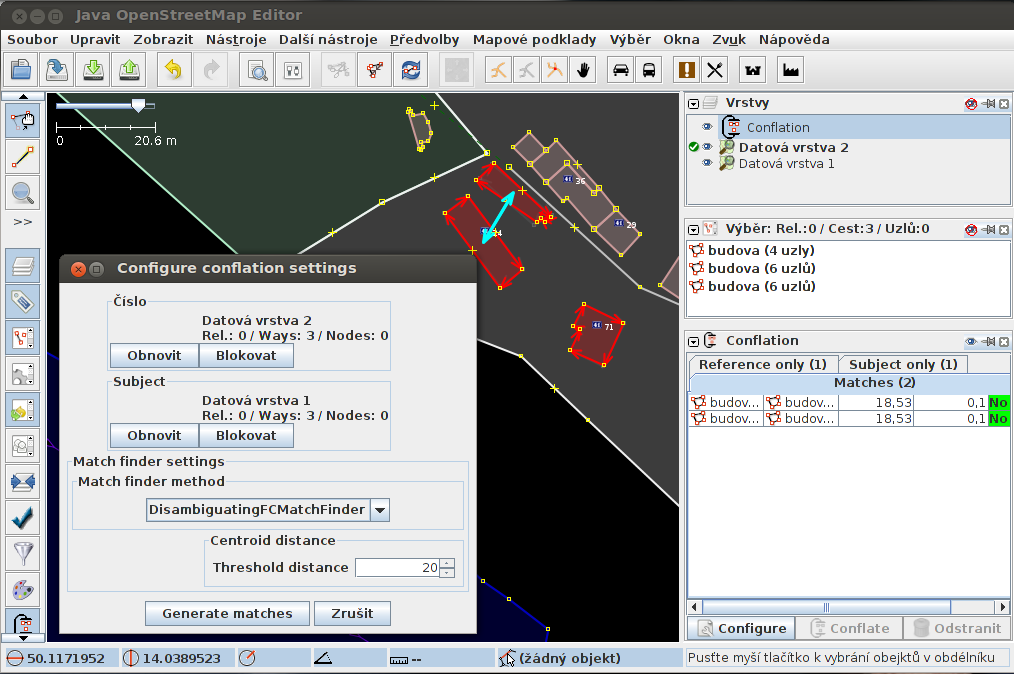
\includegraphics[width=280pt]{./pictures/josm.png}
      \caption{JOSM conflation}
      \label{fig:josm}
  \end{figure} 

V~prvním kroku je určena referenční a~upravovaná vrstva. Poté je třeba v~obou
těchto vrstvách označit prvky, které by si měly odpovídat. V~dalším kroku se 
provede automatická identifikace dvojic vybraných prvků z~obou datasetů. 
Nakonec se vykoná samotný proces zarovnání prvků (\textit{conflate}), kdy 
jsou prvky upravované vrstvy změněny tak, aby odpovídaly prvkům vrtsvy 
referenční. Jedná se o~proces poloautomatický, jelikož nejdříve je třeba
ručně identifikovat odpovídající si prvky a~teprve na~základě tohoto kroku je 
provedena automatická úprava prvků.

\subsubsection{Potlatch 2 merging tool}

\textit{Potlatch 2 merging tool} je nástroj původně navržený pro spojování 
vektorových dat cyklistických tras v~rámci England Cycling Data 
Project\footnote{Projekt pod záštitou britského ministerstva dopravy, 
který si klade za~cíl umožnit dostupnost informací o~síti cyklostezek
ve~Velké Británii prostřednictvím OpenStreetMap.}. 
V~případě tohoto nástroje se jedná především o~proces přenosu atributů. 
Pokud se v~mapě nachází dva odpovídající si prvky, pomocí tohoto nástroje je 
lze označit za~odpovídající a~jednoduše sloučit jejich atributy. Nutno 
však podotknout, že výběr odpovídajících si prvků se musí provést vždy ručně. 


\subsection{Univerzitní projekty}
\label{univerzitní}

Mimo výše uvedené nástroje existuje také několik projektů různých světových
univerzit zabývajících se buď kombinací geo\-grafických dat obecně nebo 
spojováním map silničních sítí. Možnosti využití těchto programů pro běžného
uživatele se velmi různí. A~ne vždy lze zcela volně tyto nástroje vyzkoušet. 
Jedním z~nich je i~Conflation System MBP, který byl vyvinut na~katedře počítačů 
(\textit{Computer Science Department}) na~Central Washington University v~USA. 
V~rámci tohoto projektu vznikl \textit{MBPConflate} software, který má přispět 
k~výzkumu v~oblasti slučování geo\-grafických dat. Program umožňuje automatické 
spojení map, poskytuje nástroje pro následnou kontrolu kvali\-ty výsledné mapy. 
Je navržen tak, aby bylo snadné implementovat nové techniky a~algoritmy v~této 
oblasti. Bohužel k~tomuto nástroji nejsou k~dispozici dostatečné informace týkající
se licence a~dostupnosti. 

   \begin{figure}[hbt]
     \centering
       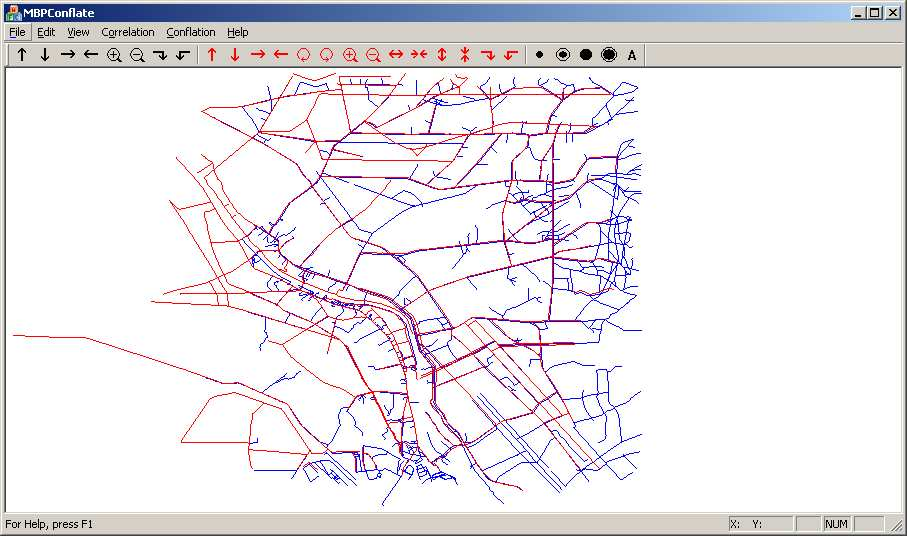
\includegraphics[width=280pt]{./pictures/MBPconflate.png}
       \caption[MBPConflate]{MBPConflate (zdroj: \cite{mbp})}
       \label{fig:mbp}
   \end{figure}
